% !TEX root =  thesis.tex
\chapter{Detailed System Description}\label{detailedSystemDescription}

\section{Design overview}

The system is broken into five major packages called application, input, output, simulation, and tasktree. Figure 5.1 shows the relationship between these components.

\begin{figure}[H]
\centering
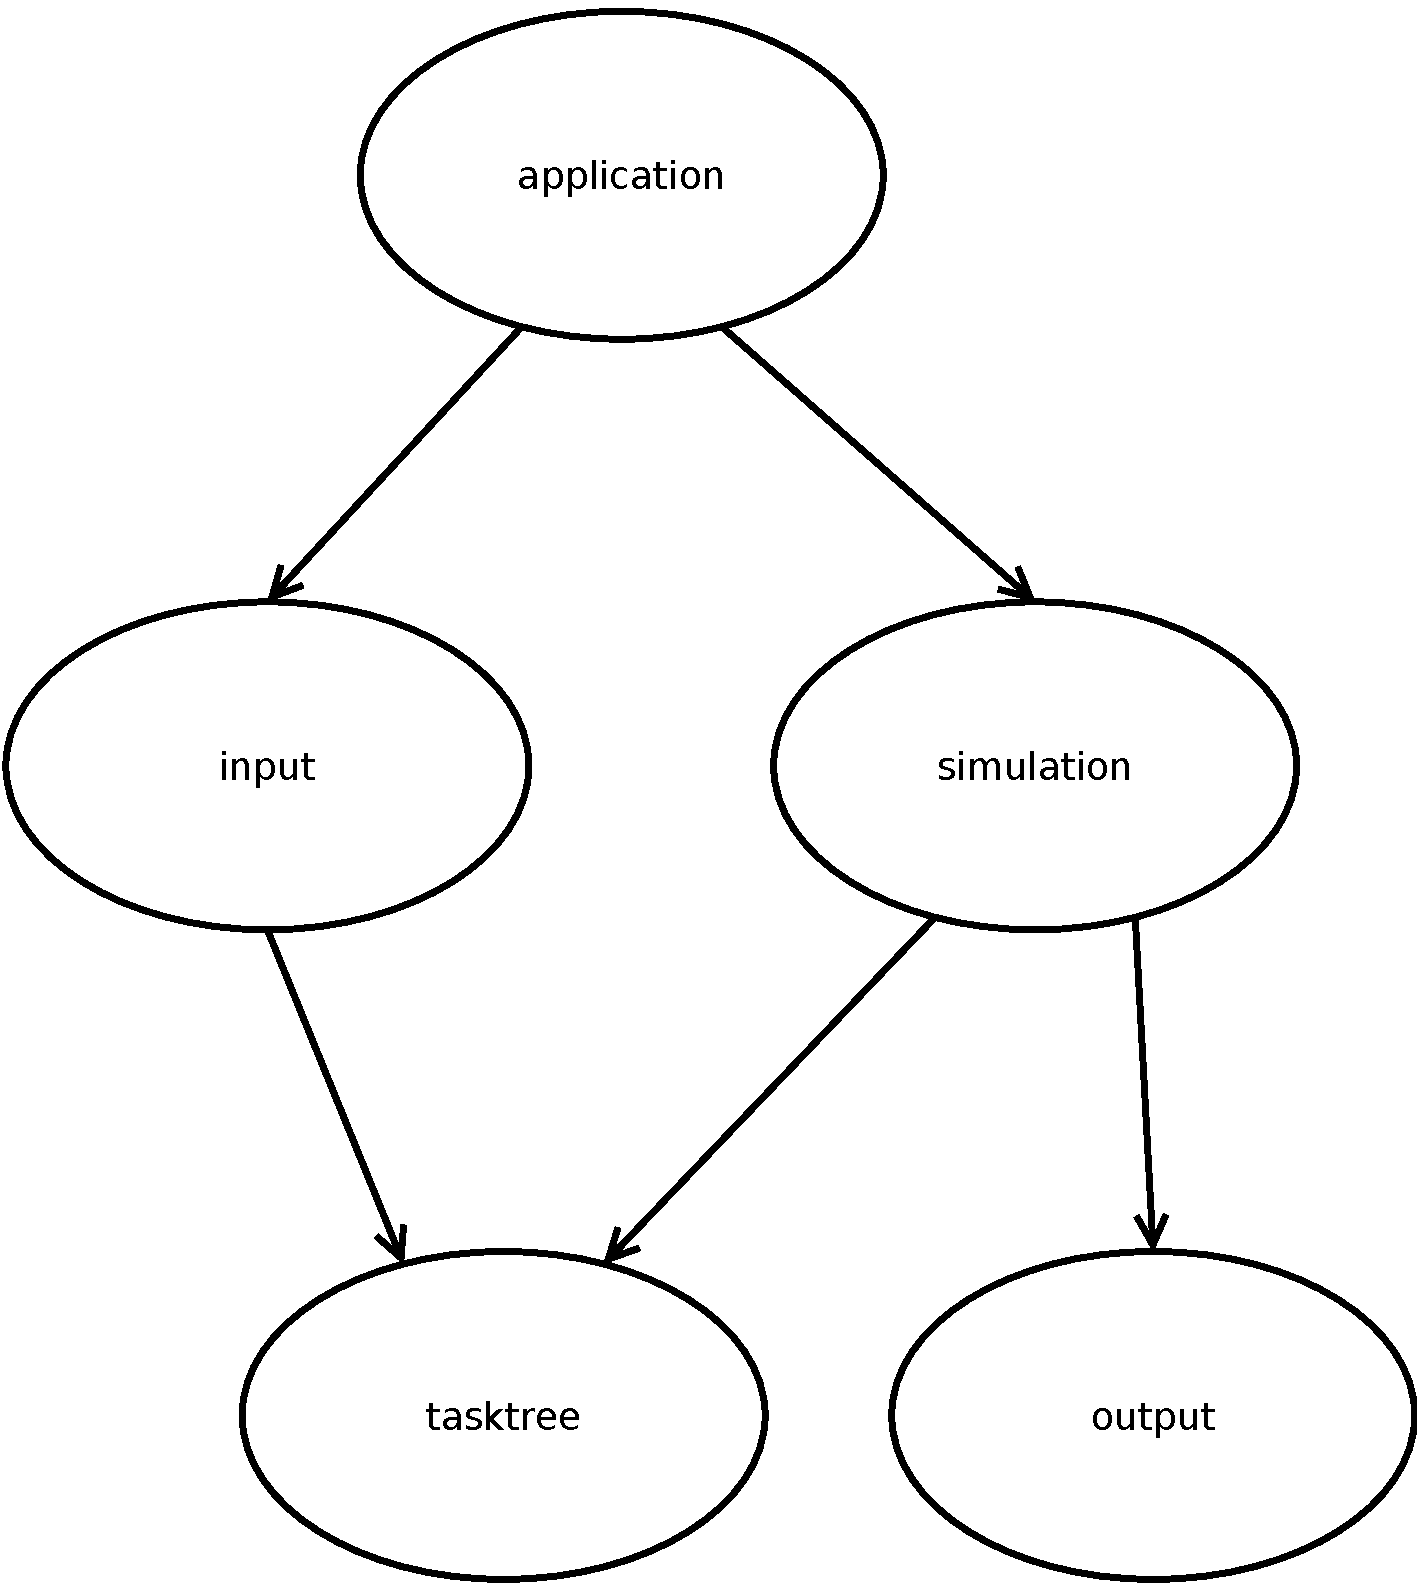
\includegraphics[trim=0.5cm 0.5cm 0.5cm 0.5cm,width=3.0in]{figs/packageUSES}
\caption{USES diagram for packages within MASS.}
\label{fig:UsesDiagram }
\end{figure}

\section{Package Overview}

\begin{enumerate}

\item\textbf{application}
\begin{itemize}
\item Description: The application package is responsible for initializing the other packages and linking everything together.
\item Contains: The application package contains module AISim.
\item Uses: This package uses the input, and simulation packages.
\end{itemize}

\item\textbf{input}
\begin{itemize}
\item Description: The input package is responsible for reading the initial data input and building a Task Tree to represent this data.
\item Contains: The input package contains three modules which include InputParser, ConfigurationParser, and FileExceptions.
\item Uses: This package uses the tasktree, and simulation packages.
\end{itemize}

\item\textbf{simulation}
\begin{itemize}
\item Description : The simulation package is responsible for connecting and communicating with agents, managing the Task Tree, and advancing the clock. Figure 5.2 represents the USES diagram for the package simulation.
\item Contains : This package contains the modules Simulator, Agent, Message and ServerThread.
\item Uses : This package uses the tasktree and output packages.
\end{itemize}

\item\textbf{tasktree}
\begin{itemize}
\item Description : The tasktree package is responsible for representing the Task Tree in a hierarchical manner that is easy for the simulation package to update and distribute.
\item Contains : This package contains the modules Node, NodeRelationship, and Distribution.
\item Uses : This package does not use any packages.
\end{itemize}

\item\textbf{output}
\begin{itemize}
\item Description: The output package is responsible for printing data after the simulation has completed. It is also responsible for logging detailed data to a file during the course of the simulation.
\item Contains: The output package contains a module Logger.
\item Uses: This package does not use any packages.
\end{itemize}

\begin{figure}[H]
\centering
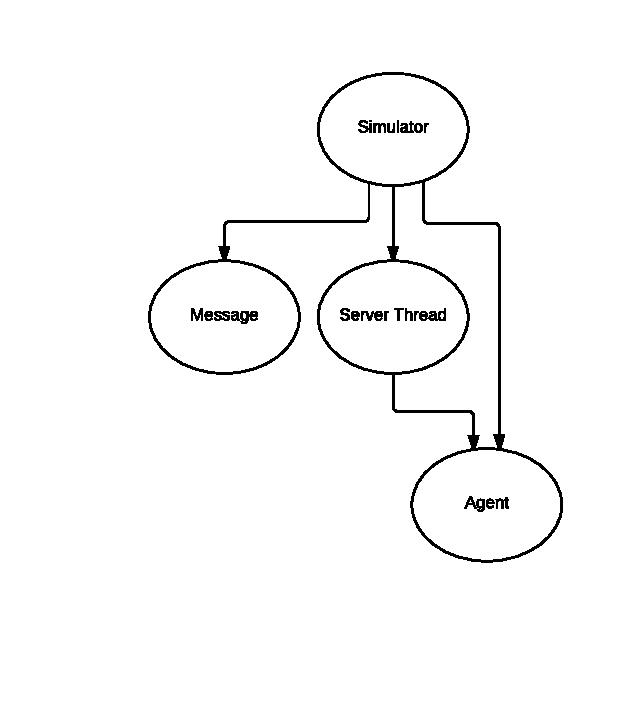
\includegraphics[trim=0.5cm 2.5cm 0.5cm 1.0cm, width=3.5in]{figs/simPackage}
\caption{Uses diagram for the package simulation}
\label{fig:simulation}
\end{figure}

\end{enumerate}

\section{Detailed Package Design}

\begin{enumerate}

\item \textbf{Application}  The application package is responsible for initializing the modules within the input and simulation packages in order to begin the Simulation.

\begin{figure}[H]
\centering
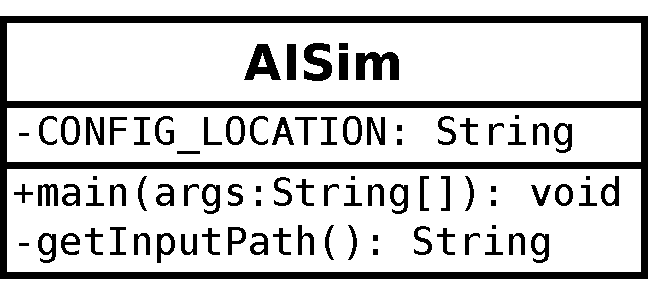
\includegraphics[width=1.5in]{figs/applicationUML}
\caption{UML diagram for input package}
\label{fig:input}
\end{figure}

\item \textbf{Input} Figure 5.3 represents the UML class diagram for input package. This package is responsible for reading and parsing the cTAEMS SFI and the plain text CFI. This packages contains an InputParser class and a ConfigurationParser class. \\

\begin{itemize}
\item \textbf{InputParser}: The InputParser is responsible for reading the SFI which contains definitions for Agents, Nodes, and Relationships that make up the Simulation. The first step of the parse involves reading the desired cTAEMS file into a string by implementing Java's BufferedReader class. Second, the string is split into tokens such as Agent, Task, Task Group, Method, and Relationship. These tokens are further parsed in order to analyse their various components. For example, a Task could be broken up into a label, list of Subtasks and QAF which are instantiated into the corresponding Task class. This data is used to build an instance of the TaskTree class which is then stored in the InputData class which will be passed to the simulation. Additionally, there are 'newtaems' tokens which may contain tasks, methods and relationships. These newtaems tokens have a time field which tells the simulation when the newtaems components will enter the simulation. Until the specified time is reached, these components will remain inactive and will be invisible to all agents. Also, newtaems tokens may add new subtasks to an existing task or taskgroup with the use of a 'splice' token. The new subtasks must be defined below this splice token or errors will be thrown by the parser. \\

\begin{figure}[H]
\centering
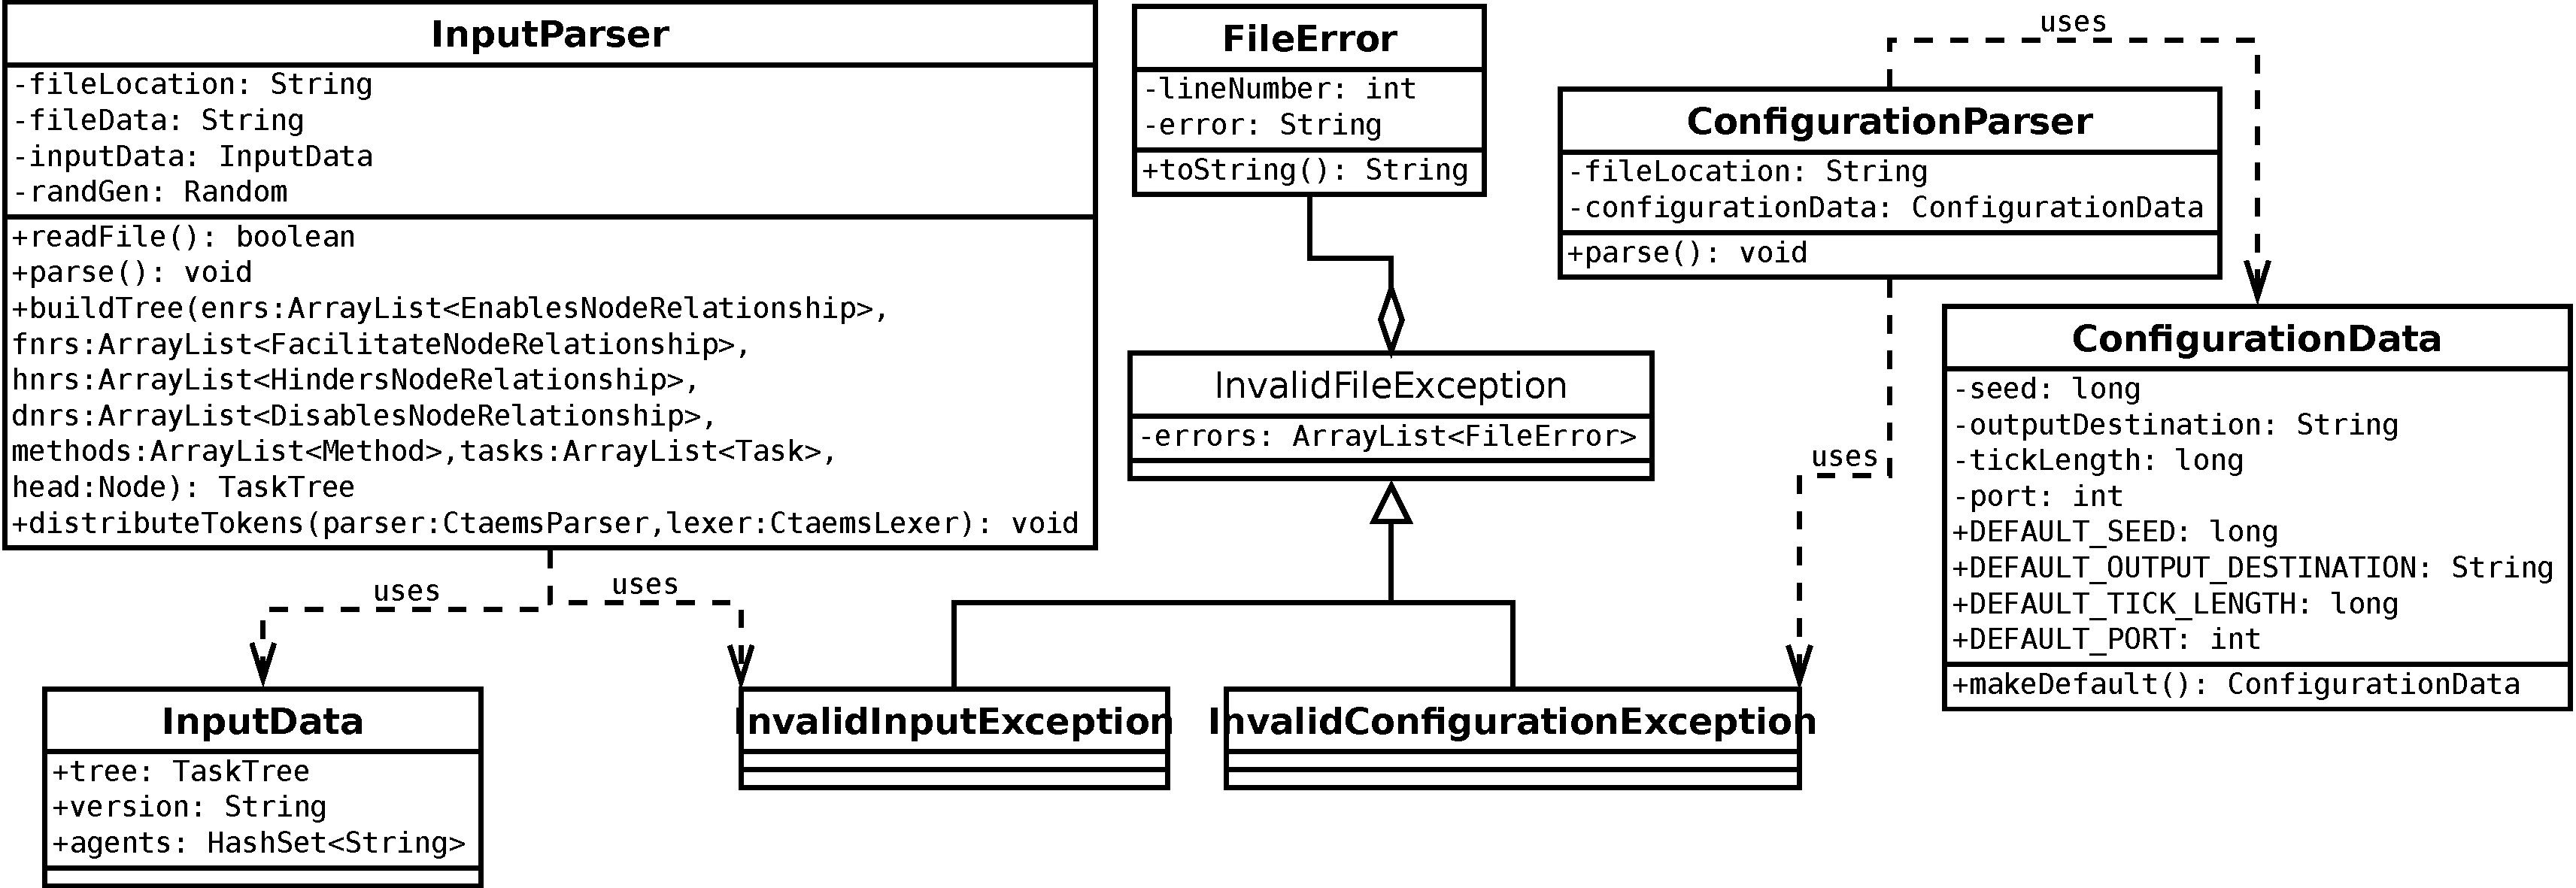
\includegraphics[width=7.0in]{figs/inputUML}
\caption{UML diagram for input package}
\label{fig:input}
\end{figure}


\item \textbf{ConfigurationParser}: The configuration parser reads and parses the CFI to determine the random seed used throughout the Simulation. The Configuration parser will use Java's Scanner class to read in the file, with each line representing one of the following seed, output destination, length of a tick, or communication port. This data is written to the ConfigurationData class which is sent to the simulator. \\

\item \textbf{Exceptions}: Within the input package there are three exceptions which are used to report a problem encountered during a parse. These exceptions are: InvalidFileException, InvalidInputException, and InvalidConfigurationException. InvalidInput and InvalidConfiguration both inherit from InavlidFile. \\
\end{itemize}

\begin{figure}[H]
\centering
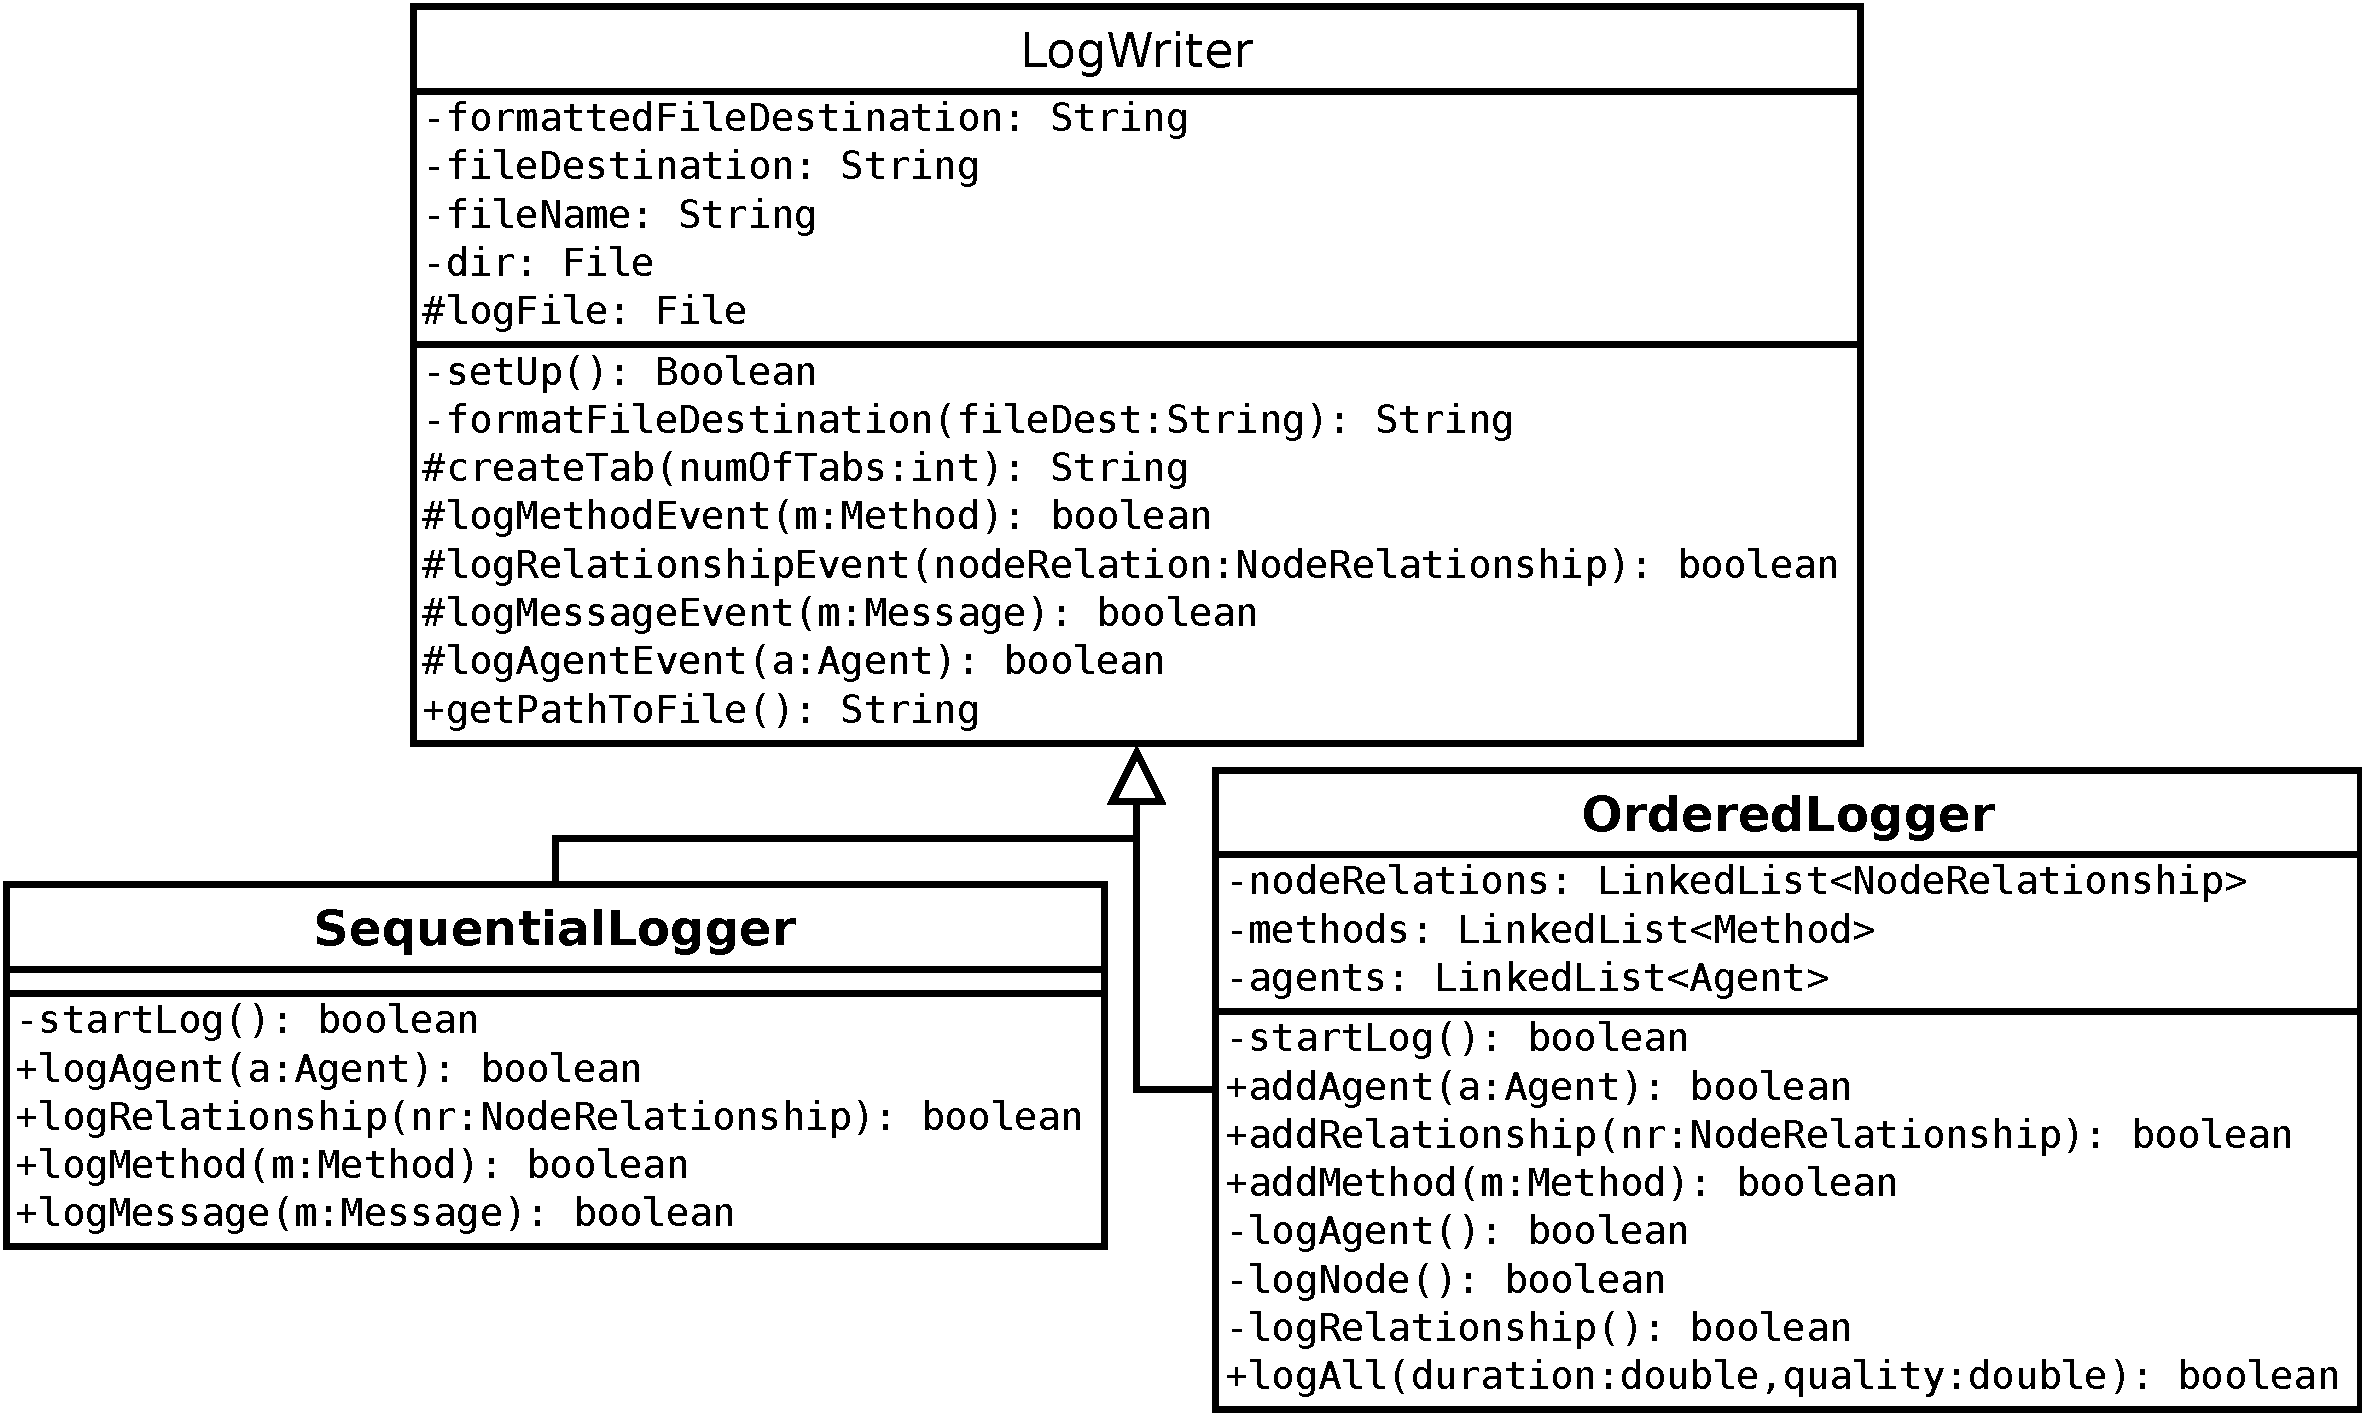
\includegraphics[width=5.0in]{figs/outputUML}
\caption{UML diagram for output package}
\label{fig:output}
\end{figure}

\item \textbf{Output} Figure 5.5 represents the UML diagram for output package. The output package is responsible for logging data after the simulation has completed. It contains a Logger class which upon completion will create the LFO document. \\

\begin{itemize}
\item \textbf{Logger}: The Logger class is responsible for producing a  transcript of Agent communication, statistics on Agent communication frequency, and the intermediate and final Quality and Duration that results from completing a Node in the Task Tree. Data will be passed to the Logger by the modules within the simulation package as the simulation advances. Upon completion of a simulation, the Logger will compile statistics on agent communication and produce the LFO containing the previously mentioned data. \\
\end{itemize}

\item \textbf{Simulation}  Figure 5.6 represents the UML diagram for simulation package. The simulation package is responsible for handling all of the communications with Agents as well as updating the Task Tree architecture to model the current state of the simulation. \\

\begin{itemize}
\item \textbf{Simulator}: This class contains all of the information about the simulation such as the random number seed, the Task Tree instance, the list of currently connected Agents, the Logger object, the list of currently running Methods, and the ServerCommunicateThread. This class is the core timekeeper of the simulation. \\

\begin{figure}[H]
\centering
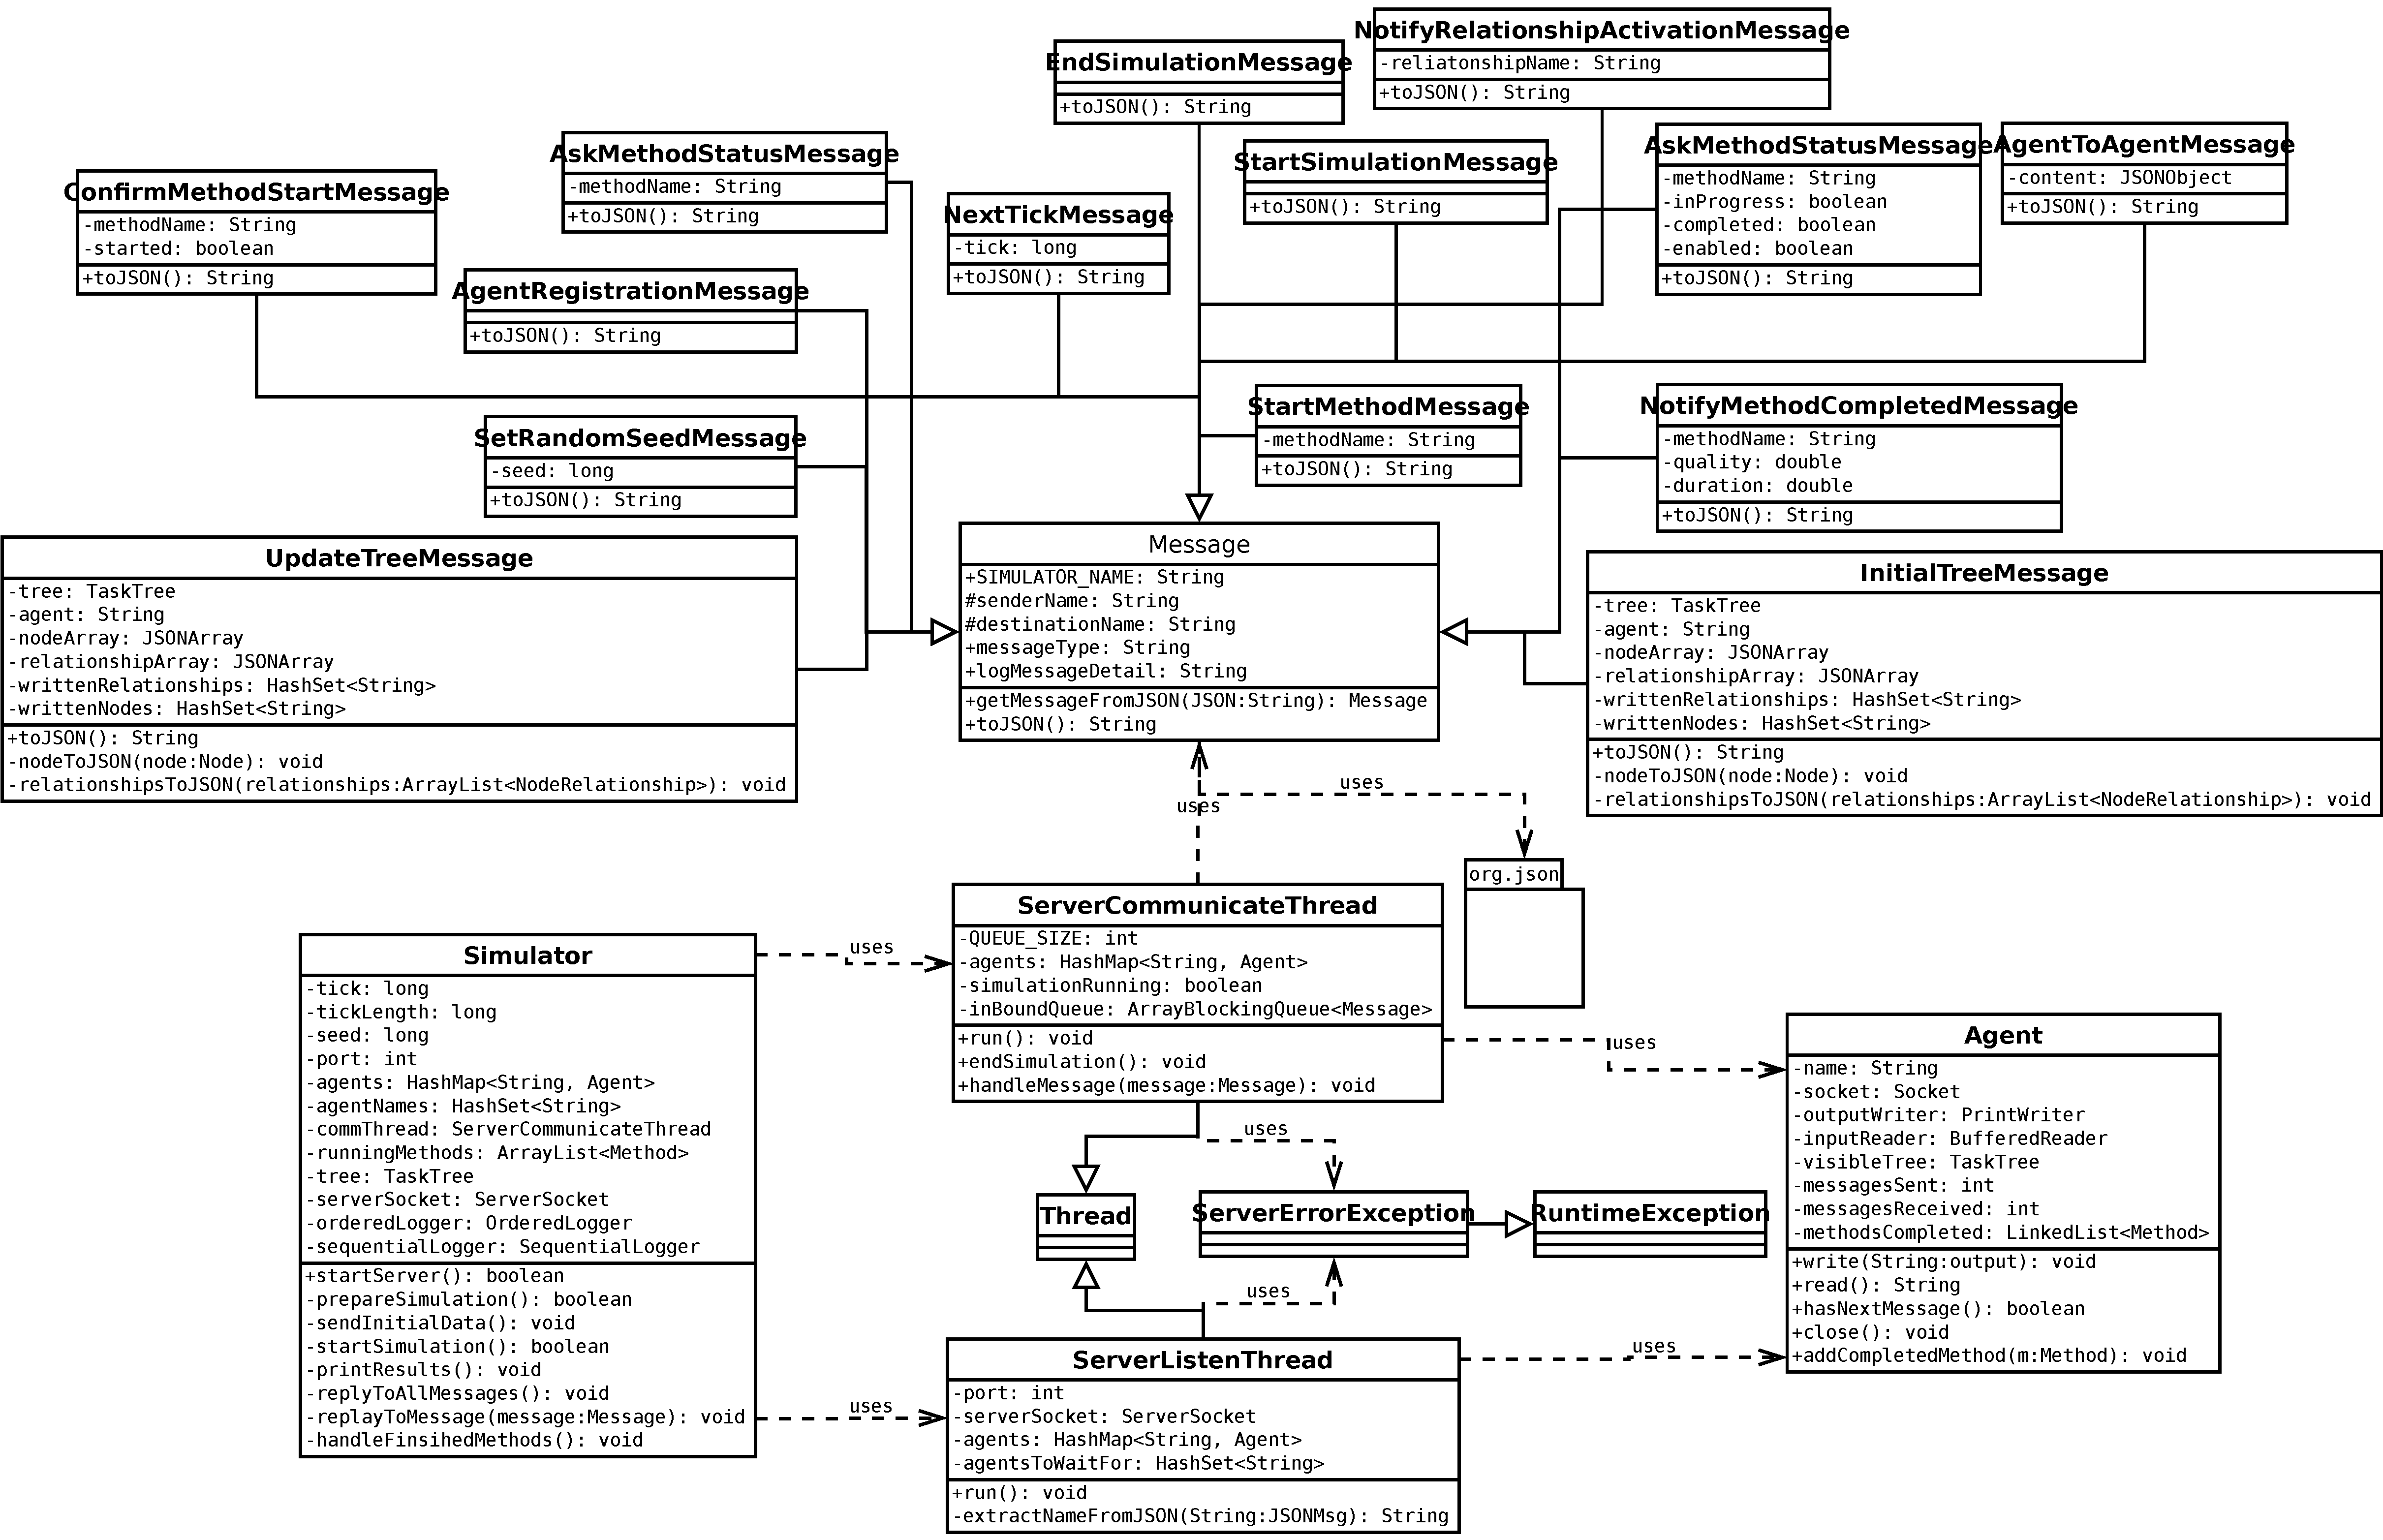
\includegraphics[width=7.0in]{figs/simulationUML}
\caption{UML diagram for Simulation package}
\label{fig:Simulation}
\end{figure}



\item \textbf{Agent}: This class is used to encapsulate all the relevant information about an Agent such as its name, and HashMap of visible Nodes. This class also contains a PrintWriter and BufferedReader that are used to communicate with the external Agent program that it represents. \\

\item \textbf{ServerListenThread}: This Thread will listen for new Agents that are trying to connect to the simulation. If an Agent connects with a valid name then this thread packages the Agent's information into an Agent object so that it can be accessed and communicated with throughout the simulation. \\

\item \textbf{ServerCommunicateThread}: This Thread will create and process all Messages coming in from and going out to all Agents in the simulation. It contains a queue of received messages that the Simulator will dump and process at the start of each tick.\\

\item \textbf{Message}: This class contains the base information for a Message such as the senderName, and the destinationName. There are many subtypes of Messages listed below. It also has a factory method to allow the creation of a new Message from a received JSON string.\\


\subitem \textbf{(i) StartMethodMessage}: Tells the Simulator that the Agent wants to start a Method.
\subitem \textbf{(ii) ConfirmMethodStartMessage}: Tells an Agent that they have successfully started a Method. 
\subitem \textbf{(iii) AskMethodStatusMessage}: Ask the Simulator for the status of a currently running Method.
\subitem \textbf{(iv) NotifyMethodStatusMessage}: Tells an Agent the status of a currently running Method.
\subitem \textbf{(v) NotifyMethodCompleteMessage}: Tells an Agent that their Method has completed and what the result is.
\subitem \textbf{(vi) InitialTreeMessage}: The Simulator tells the Agent about it's initial visible nodes.
\subitem \textbf{(vii) SetRandomSeedMessage}: Tells an Agent to set their random number seed to a specified number.
\subitem \textbf{(viii) NotifyRelationshipActivationMessage}: Tells an Agent that a NodeRelationship was activated and what the result is.
\subitem \textbf{(ix) AgentRegistrationMessage}: Ask the Simulator to register this Agent into Simulation.
\subitem \textbf{(x) StartSimulationMessage}: Tells an Agent that the simulation has started.
\subitem \textbf{(xi) EndSimulationMessage}: Tells an Agent that the simulation has ended.
\subitem \textbf{(xii) NextTickMessage}: Tells an Agent about a new tick.
\subitem \textbf{(xiii) UpdateTreeMessage}: Gives new TaskTree data to an Agent.
\subitem \textbf{(xiv) AgentToAgentMessage}: Sends a JSON object from one Agent to another Agent and the implementation of the Agents is responsible for filling out that object and interpreting it.\\
\end{itemize}

\begin{figure}[H]
\centering
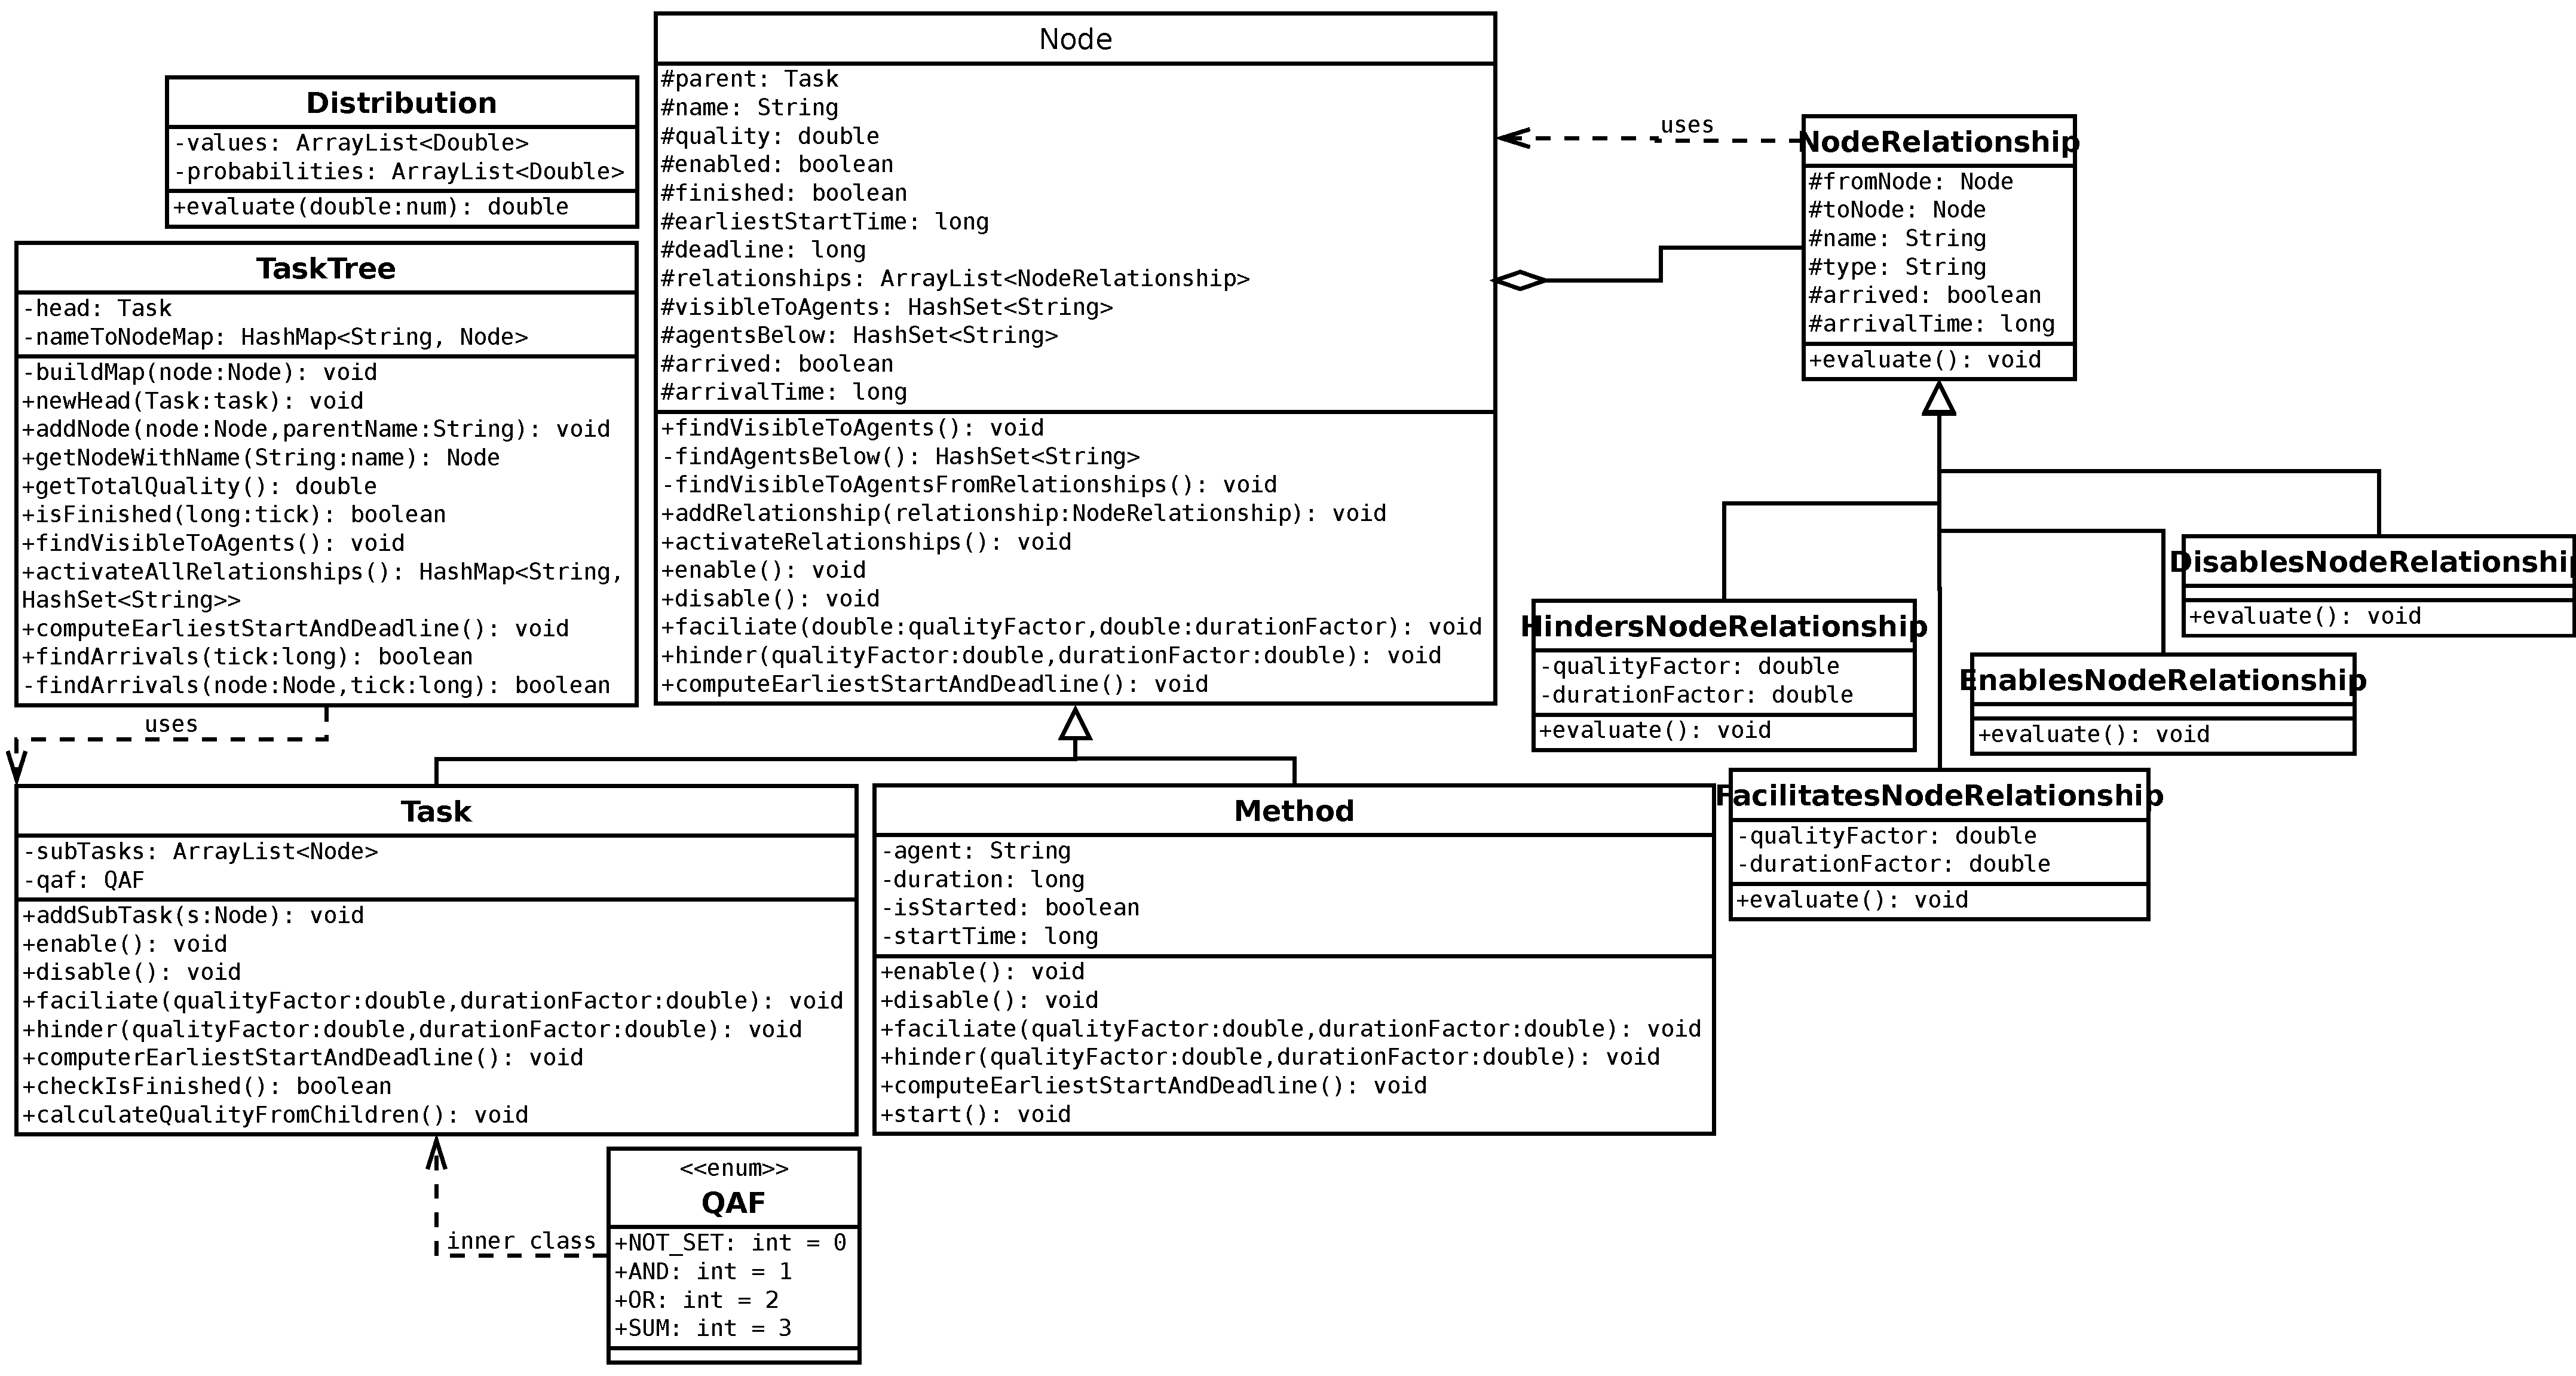
\includegraphics[width=7.5in]{figs/tasktreeUML}
\caption{UML diagram for tasktree package}
\label{fig:TaskTreeUML}
\end{figure}

\item \textbf{Tasktree} This package provides a framework for building a Task Tree. It is used by the input package to construct a programmatic representation of the SFI including Task, Methods, and Node relations. \\

\begin{itemize}

\item \textbf{TaskTree}: A wrapper class for the whole Task Tree. Contains a reference to the head Node of the tree. Also contains some methods to allow easily information gathering about the tree.

\item \textbf{Node}: The base Node class that contains all the information about a Node of the tasktree such as Quality, name, this Nodes parent Node, a list of NodeRelationships from this Node, whether or not the Node is enabled, and whether or not the Node is finished. \\

\item \textbf{Task}: A Task is a type of Node whose completion is defined by its Subtasks. A Task's completion quality is the result of it's QAF being run. More Quality options can be added as needed. A Subtask can either be another Task which would have more Subtasks or a Method which has no Subtasks. \\

\item \textbf{Method}: A Method is a Node that can be completed by a specific Agent. The Method contains a Duration which is the amount of time it takes to complete the Method. Methods can have their Duration and Quality modified by the FacilitatesNodeRelationship and HindersNodeRelationship. \\

\item \textbf{NodeRelationships}: There are many NodeRelationships that represent the affect that the completion of one Node has on another. The types of NodeRelations are below. \\

\subitem \textbf{(i) HindersNodeRelationship}: Completing one Node decreases the Quality and increases the Duration of a Method.

\subitem \textbf{(ii) FacilitatesNodeRelationhip}: Completing one Node increases the Quality and decreases the Duration of a Method.

\subitem \textbf{(iii) EnablesNodeRelationship}: The completion of the first Node enables the starting of the second Node

\subitem \textbf{(iv) DisablesNodeRelationship}: The completion of the first Node disables the starting of the second Node.

\item \textbf{Distribution}  A Distribution is used to generate Qualities and Durations for the Nodes. It is given a probability distribution specified in the cTAEMS file and a random number. The Distribution then calculates which value it should return.


\end{itemize}
\end{enumerate}